\section*{Design}\label{design}

% System Architecture (Your idea)
% • Prototyping (how you implemented it)
% • Testing (how you are going to test it → Result)

\subsection{Architecture}\label{architecture}

\begin{figure}[h]
  \begin{center}
    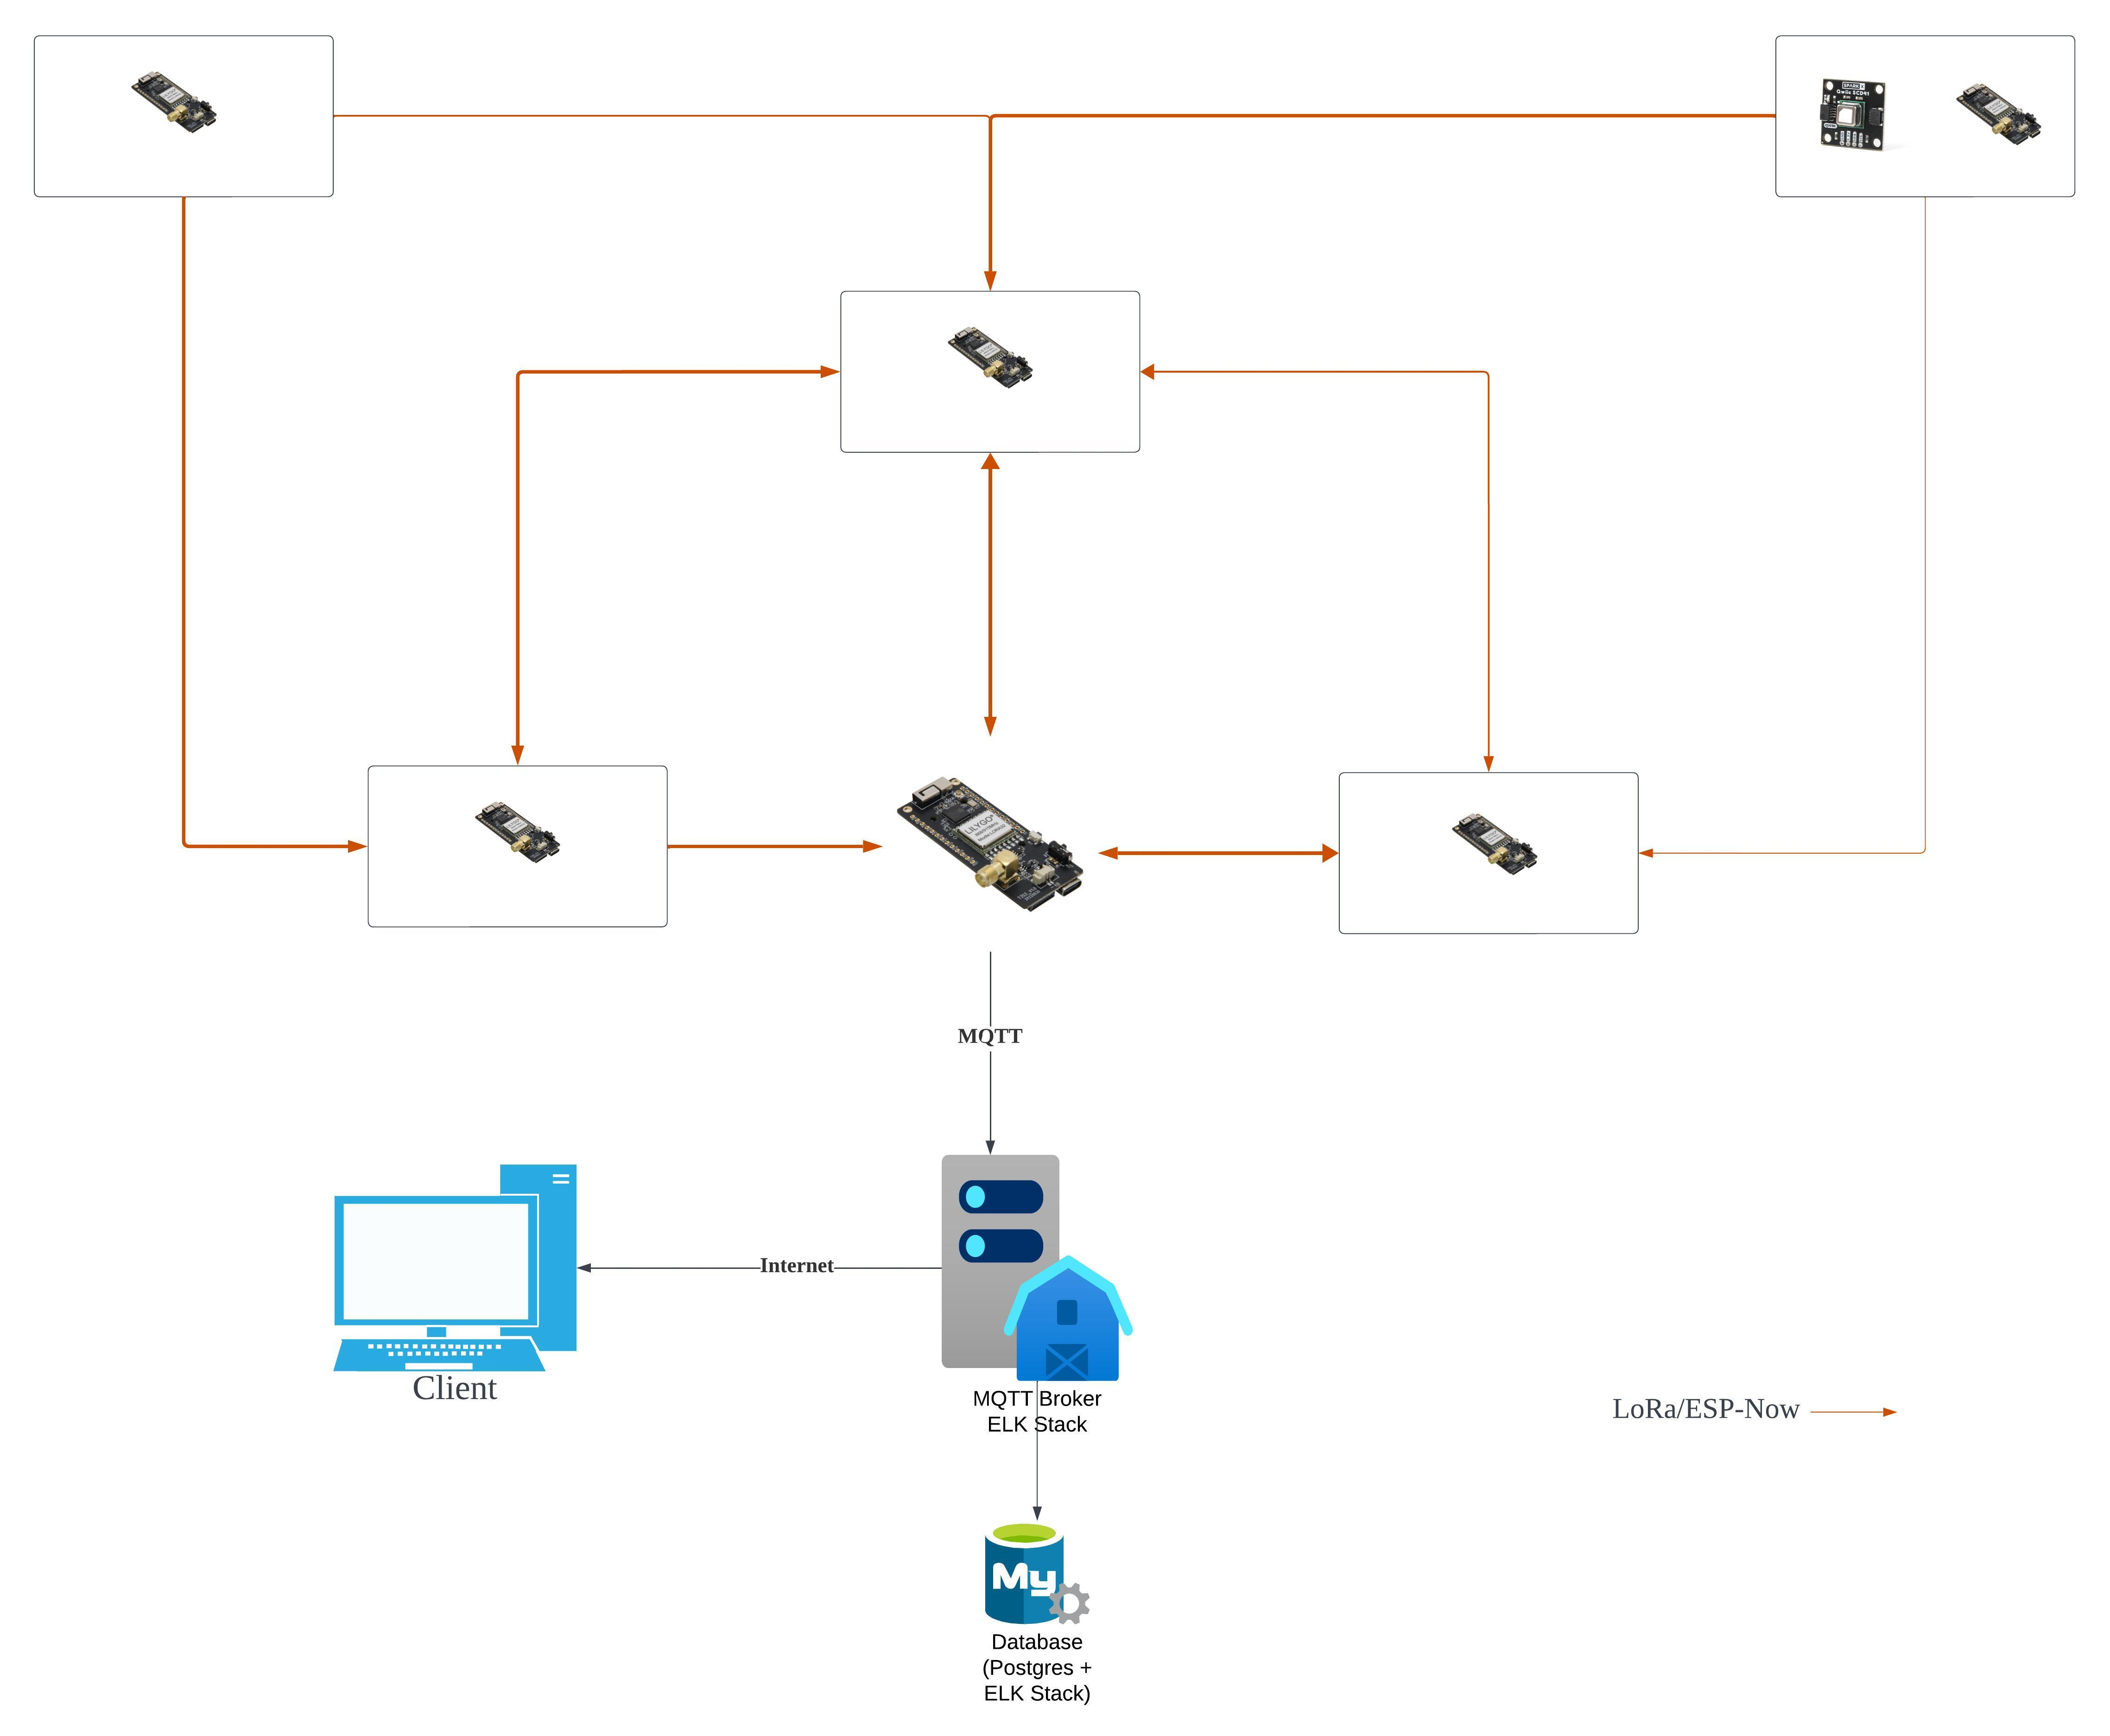
\includegraphics[width=0.35\textwidth]{architecture.jpeg}
  \end{center}
  \caption{Proposed System Architecture}\label{architecture}
\end{figure}

Our system architecture aims to streamline data collection and analysis from a Wireless Sensor Network (WSN) Mesh, comprising two main components: the WSN Mesh itself and the data collection sink. Sensor nodes equipped with the Liligo T3S3 Lora 2.4Ghz module form the WSN Mesh, communicating via ESP=Now and LoRa Protocols for efficient node discovery and routing. The root node establishes a secure MQTT connection with the sink, responsible for aggregating data from the WSN Mesh and forwarding it to the ELK Stack for visualization and analysis.

\subsection{Prototyping}\label{prototyping}
For prototyping, we plan to deploy sensor nodes with the Liligo T3S3 Lora 2.4Ghz module, utilizing ESP-Now and LoRa Protocols for communication. One node interfaced with the SCD41 Sensor, while others generated synthetic data. The root node connected to the sink via MQTT, ensuring seamless data collection, analysis and visualisation. As an enhancement, we plan to implement protocol switching to adapt to varying network conditions.

\subsection{Testing}\label{testing}
To validate our system, we conducted unit testing on sensor nodes to ensure proper communication and data generation. Integration testing confirmed the WSN Mesh's interoperability and data transmission to the sink. Stress testing evaluated scalability and resilience under heavy loads. Results demonstrated successful communication within the WSN Mesh, reliable data transmission to the sink, and system robustness, meeting deployment requirements.

